\documentclass[fleqn]{article}

\usepackage[utf8]{inputenc}
\usepackage{cite}

\usepackage{amsfonts}
\usepackage{amsmath}
\usepackage{amssymb}

\usepackage{hyperref}
\usepackage{syntax}
\usepackage{listings}
\usepackage{zed-csp}


\usepackage{tikz}
\usetikzlibrary{positioning}

\lstdefinelanguage{sal}{
  keywords = {send, become, let, new, in, to, if, then, else, case, def, end,
    case, of, ||}
}

\lstdefinelanguage{csp}{
  keywords = {channel, datatype}
}

\lstdefinestyle{simple}{
  basewidth=0.5em
}

\newcommand{\SAL}{\textbf{SAL}}

\title{CSP}
\author{José Luis Diaz}
\date{ }
 
\begin{document}
 
\maketitle
 
\tableofcontents
 
\section{Introducción}

\section{Conceptos básicos}

\subsection{Comportamientos} \label{comportamientos}

\subsection{Creando Actores}

\subsection{Creando comunicaciones}

\subsection{Comandos}

\section{Lenguaje de Actor Mínimo}

Un programa en \SAL no es mas que una secuencia de \textit{comportamientos}.
Como en la mayoría de los lenguaje de programación, tiene un nombre reservado
\textbf{main}, este \textit{Comportamiento} es el punto de entrada, será el
responsable de crear otros actores y enviar mensajes.

\begin{grammar}
   <Pgm> :== $BDef_1 ... BDef_n BDef_{main} $ 
\end{grammar}

la definición de \textit{comportamientos} funcionan como una suerte de plantilla
para el comportamiento que luego tendrán los actores. 

\subsection{Expresiones}
Existen tres tipos primitivos, booleanos, enteros y dirección del buzón. Las operaciones
posibles entre los booleanos son \textbf{or}, \textbf{and}, \textbf{not}. Con
respecto a los enteros se pueden operar utilizando \textbf{+}, \textbf{-},
\textbf{*}, \textbf{/}. Un buzón es un identificador que es devuelto cuando se
crea un nuevo actor.

\subsection{Definición de comandos}
La gramática de los comandos en SAL es la siguiente:

\begin{grammar}
  <command> ::= `send' $e_1, e_2, \ldots\ , e_n$ `to' <actor>  
  \alt `become' $B(e_1, e_2, ..., e_n)$
  \alt `let' $x_1$ = `new' $B_1(e_1, e_2, ..., e_{1n})$, \\
   \ldots\ \ $x_k$ = `new' $B_k(e_1, e_2, ..., e_{kn})$       \\
  `in' <command> 
  \alt `if`<bool-expr> `then' <command> `else' <command> `end if'
  \alt <command> `||' <command>
\end{grammar}

\begin{description}
\item [send]  Este comando permite enviar mensajes a otros actores, toma como
  parámetro una lista separada por coma de las expresiones a enviar, y el actor
  destino, el envío de mensajes es asincrónico. Cada expresión es evaluada antes
  de ser enviada.
\item [become] Este comando especifica el siguiente comportamiento del actor
  que está procesando la comunicación recibida. Como en el caso anterior se evalúan
  las expresiones antes de ser enviadas, y estas aparecerán como la listas de
  parámetros del comportamiento. 
\item[new] Este comando sirve para crear nuevos actores. El alcance de los
  identificadores de los nuevos actores creados está sujeto al cuerpo de \textbf{let}.
\item[condicional] Luego de evaluar la expresión booleana, si es verdadera
  ejecuta lo que esta a continuación de \textbf{then}, en caso contrario lo que está a
  continuación de \textbf{else}. Funciona como cualquier condicional.
\item[composición] Estos dos comandos en \SAL son ejecutados concurrentemente.
 
\end{description}

La ejecución de los comandos ocurre cuando el actor recibe un mensaje, y todos
ellos ocurren concurrentemente, la composición no es secuencial.

\subsection{Definición de comportamientos}

La sintaxis de los comportamientos es la siguiente:

\begin{grammar}
 <BDef> :== `def' <beh name> `(' <acquaiantence-list> `)' `[`'<input-list>`]' \\
  \quad <command>* \\
  `end def'
  \alt <acquaiantence-list> :== <id> | <id>`,' <acquaiantence-list>
  \alt <input-list> :== <id> | <id>`,' <input-list>
\end{grammar}

El identificador \textit{beh name} esta atado a una abstracción y tiene alcance
a todo el programa. Los identificadores \textit{acquaiantence-list} los recibe el
momento de instanciación y tiene alcance en todo \textit{command}. Los
identificadores \textit{input-list} son completados al momento de recibir un
mensaje, y su alcance es todo \textit{command}.
Ambas listas, \textit{input-list} y \textit{acquaiantence-list} contienen todos
los identificadores libres que están en \textit{command}. Existe un
identificador especial \textit{self} que puede ser utilizado para hacer
referencia al actor que está se definiendo.
La ejecución de \textit{command} deberá contar a lo sumo con un solo comando
\textit{become}, esta propiedad tiene que ser estáticamente garantizada, de no
existir nigún comando \textit{become}, el actor asumirá un comportamiento de
tipo \textit{bottom}, es es básicamente ignorar los mensajes que se le envíen.

\subsection{Ejemplo}

Está implementación del factorial está adaptada de \cite{Agha:1986:AMC:7929}, esta
depende de un actor \textit{main} que le envía el valor a calcular. El factorial
esta siempre disponible para procesar la siguiente comunicación, no bloquea con
el calculo recursivo del factorial sino que lo delega en otros actores.

La palabra reservada \textit{self} hace referencia a la dirección de buzón
correspondiente al actor que está procesando la comunicación, este es inicializado
cuando el actor es creado.

\begin{lstlisting}[language=sal, style=simple]
def Factorial()[val, customer]
  become factorial() ||
  if val = 0 then
  send [1] to customer
  else
    let cont = new FactorialCont(val, customer)
       in send [val - 1, cont] to self
  end if 
end def

def FactorialCont(n, customer)[arg] 
  send [n * arg] to customer
end def
\end{lstlisting}

El actor ante un entero distinto de cero ejecuta dos acciones, crea un actor con
un comportamiento que será multiplicar por \textbf{n} el valor recibido y
enviarlo al buzón de quien pidió el calculo del factorial de \textbf{n}.
También, se envía un mensaje a si mismo para evaluar el factorial de \textbf{n -
  1}, y como dirección de cliente utiliza la dirección del buzón del actor
recientemente creado. Este comportamiento se puede ver en la figura \ref{fig:factorial}.
En caso de que reciba \textbf{0} se le enviara \textbf{1} a quien pidió el
calculo del factorial.

\begin{figure}
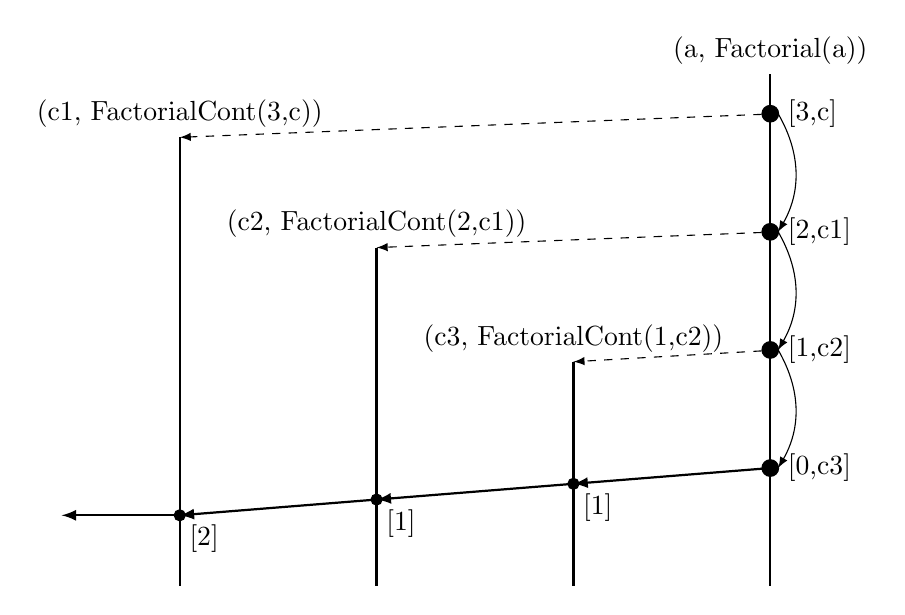
\begin{tikzpicture}
\draw[thick] (8,7) -- (8, 0.5);

\node[] (a1) at (8,7.3) {(a, Factorial(a))};

\node[align=center, right] (a1) at (8.1,6.5) {[3,c]};
\draw[fill] (8,6.5) circle (3pt);

\node[align=center, right] (a2) at (8.1,5) {[2,c1]};
\draw[fill] (8,5) circle (3pt);

\node[align=center, right] (a3) at (8.1,3.5) {[1,c2]};
\draw[fill] (8,3.5) circle (3pt);

\node[align=center, right] (a4) at (8.1,2) {[0,c3]};
\draw[fill] (8,2) circle (3pt);

\draw[-latex] (a1.west) to[bend left] (a2.west);
\draw[-latex] (a2.west) to[bend left] (a3.west);
\draw[-latex] (a3.west) to[bend left] (a4.west);

\node[] (d1) at (0.5,6.5) {(c1, FactorialCont(3,c))};
\draw[thick] (d1.south) -- (0.5, 0.5);

\node[] (c1) at (3,5.1) {(c2, FactorialCont(2,c1))};
\draw[thick] (c1.south) -- (3, 0.5);

\node[] (b1) at (5.5,3.65) {(c3, FactorialCont(1,c2))};
\draw[thick] (b1.south) -- (5.5, 0.5);


\draw[fill] (5.5,1.8) circle (2pt);
\node[align=center, right] (b2) at (5.5,1.5) {[1]};

\draw[fill] (3,1.6) circle (2pt);
\node[align=center, right] (c2) at (3,1.3) {[1]};

\draw[fill] (0.5,1.4) circle (2pt);
\node[align=center, right] (d2) at (0.5,1.1) {[2]};

\draw[-latex, thick] (8,2)  -- (5.5,1.8);
\draw[-latex, thick] (5.5,1.8) -- (3,1.6);
\draw[-latex, thick] (3,1.6) -- (0.5,1.4);
\draw[-latex, thick] (0.5,1.4) -- (-1,1.4);

\draw[-latex, black, dashed] (a1.west) -- (d1.south);
\draw[-latex, black, dashed] (a2.west) -- (c1.south);
\draw[-latex, black, dashed] (a3.west) -- (b1.south);

\end{tikzpicture}
\caption{El diagrama ilustra el cálculo del factorial de 3, todo el resultado es
enviado al actor \textit{c}. Las lineas en punto indican la creación de un actor.}
\label{fig:factorial}
\end{figure}

Falta contar como funciona.

\begin{lstlisting}[language=sal, style=simple]
def stack-node(content, link)
  [ case operation of
        pop : (customer)
        push : (new-content)
    end case ]
  if operation = pop then
    become link
    send content to customer
  enf if
  if operation = push then
    let P = new stack-node(content, link)
    { become new stack-node(new-content, P) }
  end if
end def
\end{lstlisting}

\section{Un modelo en CSP}
Para empezar a describir como se modeló en CSP, primero es importante hacer
referencia a que se utilizó \textit{CSPm} \cite{fdr}, que combina los operadores de \textit{CSP}
originalmente propuesto por Hoare\cite{Hoare:1978:CSP:359576.359585}, y un lenguaje funcional.

En el proceso de traducción de \textit{SAL} a \textit{CSPm}, fue necesario construir un pequeño
\textit{runtime} para emular como los actores corren. Recordemos que la
naturaleza de \textit{CSP} es síncrona y los actores no lo son. Fue necesario
concretamente desacoplar la creación de nuevos actores, y el proceso de comunicaciones. 

Como se comentó en la sección \ref{comportamientos}, un actor puede crear nuevos actores, enviar
mensajes y debe definir su próximo comportamiento.

\subsection{Estructuras de apoyo}

\subsubsection{Enteros pequeños}

Para evitar la explosión de estados que causa utilizar todo el rango de enteros,
para el envio de mensajes se creo una abstración que minimiza la cantidad de
enteros en uso.

\[
  datatype\ SmallInt = SI.\{0 \ldots MAX\_INT\} | Overflow
\]

A continuación definimos las operaciones básicas sobre los enteros

\[
  add(SI.a, SI.b) = \\
  \quad let\ sum\ =\ a + b\ within\ if\ sum <= MAX\_INT\ then\ SI.sum\ else\ Overflow \\
  sub(SI.a, SI.b) = \\
  \quad let\ sub\ =\ a - b\ within\ if\ sub >= 0\ then\ SI.sub\ else\ Overflow \\
  mult(SI.a, SI.b) = \\
  \quad let\ mult\ = a * b\ within\ if\ mult <= MAX\_INT\ then\ SI.mult\ else\
  Overflow \\
  eq(SI.a, SI.b)\ =\ a == b \\
  eq(\_, \_)\ =\ false\\

\]

\subsubsection{Identificadores de actores}

Esta construcción nombra cada uno de los actores que van ser utilizados, también
guarda la cantidad de actores de un tipo dado. Para la definición usa tipos algebraicos
similares a los de Haskell soportados por \textit{CSPm}.

\[
  datatype\ ActorID = ACTOR_1.\{1 \ldots N_1\} | \\
  ACTOR_2.\{1, \ldots ,N_2\} | \\
  ACTOR_k.\{1, \ldots, N_k\} | \\
  Main.\{1\}
\]

El valor que está entre llaves corresponde a la cantidad de elementos de este
tipo que van a ser necesarios. Ya que no existe en \textbf{CSP} el concepto de
instancia, es necesario contar con todos los procesos al principio de la
simulación, este tipo de datos ayudará a crear los procesos necesarios como
veremos en la sección siguiente.

\subsubsection{Valores primitivos}

Ademas de los mostrados tipos de valores posibles existe una última construcción
que representa una suerte de cadena caracteres.

\[
  datatype\ Atoms = ATOM_1 | ATOM_2 | \ldots | ATOM_n
\]



\[
  datatype\ VALUE = ACTOR.ActorID | INT.SmallInt | ATOM.Atoms | None
\]

\subsection{Buzón}

Para desacoplar el envío de mensajes utilizamos una estructura intermedia que
actúa de \textit{buzón}, para comunicarase con esta estructura existen dos canales.

\[
channel\ CommSend:ActorID.(VALUE, VALUE)\\
channel\ CommRecv:ActorID.(VALUE, VALUE)
\]

Un \textit{buzón} puede guardar más de una comunicación en su interior. Esto
introduce un tipo de no determinismo ya que un actor puede sincronizar con cualquiera
de las comunicaciones disponibles en su \textit{buzón}.

El comportamiento del proceso buzón depende de su estado, si no tiene ningún
mensaje, si tiene algunos mensajes, o si está completo.
\begin{itemize}
\item Si no tiene ningún mensaje, solo sincroniza mensajes por el canal $CommSend$.
\item Si tiene algunos mensajes, por los canales $CommSend$ y $CommRecv$.
\item Si está completo, solo por el canal $CommRecv$.
\end{itemize}

Puede que los nombre de los canales suenen poco intuitivos, es importante notar que
provienen de la acciones vista desde los actores.

\begin{description}
\item [CommSend] Canal utilizado para comunicar desde cualquier actor hacia el buzón.
\item [CommRecv] Canal utilizado para comunicar del buzón hacia el actor asociado.
\end{description}

\[
mailbox(i, \nil) = CommSend?i.x \then mailbox(i, \trace{x}) \\
mailbox(i, \trace{x}) = \\
\qquad CommRecv!i.x \then mailbox(i, \nil) \Extchoice \\
\qquad CommSend?i.y \then mailbox(i, \trace{x, y}) \\
mailbox(i, \trace{x, y>}) = \\
\qquad CommRecv!i.x \then \\mailbox(i,\trace{y}) \Extchoice\\
\qquad CommRecv!i.y \then mailbox(i, \trace{x}) 
\]

Por cada actor en la red, existe un \textit{buzón} con el mismo \textbf{ActorId}
asociado a este. 
Un actor se bloquea esperando en $CommRecv$, cuando una nueva comunicación está
dispuesta a ser sincronizada, desde el \textit{buzón} hacia el actor esta es procesada.

\[
mailboxes  = \Interleave_{actor : ActorID} mailbox(actor, \nil) 
\]

$mailboxes$ representa todos los buzones puestos en paralelo utilizando el
operador de \textit{Interleave}. Como no existe comunicación entre buzones,
siempre la comunicación es desde un actor hacia un buzón  el operador
de \textit{Interleave} es el adecuado para capturar este efecto.


\subsection{Crear nuevos actores}

Antes de empezar, un ejemplo para entender como funciona un aspecto fundamental
de los canales de \textbf{CSPm}. 

\[
V = \{1,2,3\} \\
channel C:V.V \\
P1 = C?x!2 \then \Stop \\
P2 = C!1?y \then \Stop \\
SYSTEM = P1 \Parallel P2
\]

Del ejemplo anterior podemos ver que el canal \textbf{C} genera el alfabeto de
comunicación $\{ C.1.1, C.1.2, C.1.3, C.2.1, C.2.2, C.2.3, C.3.1, C.3.2, C.3.3 \}$.
En $P1$ tenemos la variable libre $x$ y en $P2$ tenemos la variable libre $y$,
es simple notar que al utilizar \textbf{`?'} podemos introducir el uso de una
variable libre, no así cuando utilizamos \textbf{`!'}.
Esto genera la sensación de poder enviar un mensaje utilizando \textbf{!} y
recibirlo usando \textbf{?}.

Recordemos que en \textbf{CSP} no existe el concepto de instancia, y debemos
tener definida la red de actores desde el comienzo.
Por esto mismo en la creación de nuevos actores nos vamos a encontrar con dos
partes involucradas, quien está iniciando un nuevo actor, y el actor que está
siendo iniciado.

\[
channel\ CreateAsk:ActorID.(VALUE, VALUE)\\
channel\ Create:ActorID.(VALUE, VALUE)
\]

Para separar el actor que tiene la intención de crear otro del que efectivamente
va a ser iniciado, el primero espera a sincronizar en un evento del tipo
$CreateAsk$, como existe un proceso auxiliar que está dispuesto encontrase con
el, se libera y así puede continuar el proceso que crea el nuevo actor.
En realidad, la creación es algo ficticio ya que tenemos una red de
procesos \textit{CSP} esperando el evento $Create$ para arrancar con el
comportamiento definido.

\[
create(actorId) = CreateAsk!actorId?m \then Create.actorId!m \then STOP
creates = \Interleave_{actor : ActorID} create(actor)
\]

\[
actors_k = \Interleave_{id : actor_k } Create!id?(p1, p2) \then
comportamiento_k(actorId, p1, p2)
\]

\subsection{Definición de comportamientos}
La idea de comportamiento fue introducida en la sección XXX, podemos pensar a un
comporamiento como una función que procesa una comunicación y tiene como salida,
nuevas comunicaciones, nuevos actores y el comportamiento de reemplazo para el
actor que esta procesando la comunicación.

ara mostrar como funciona se utilizará un ejemplo simple, un actor que cuando
es creado recibe un parámetro del tipo \textbf{ActorId}, luego se queda esperando un
mensaje, cuando lo recibe, incrementa en uno el valor que este y lo envía al buzón de $a1$.

\[
  g = Create!G.1?(a1, None) \then g_{running}(G.1, a1) \\ 
g_{running}(self, ACTOR.client) = \\
\quad CommRecv.self!(INT.v, None) \then \\
\quad CommSend.client!(add(v, SI.1), None) \then \\ 
\quad g_{running}(self, ACTOR.client) \\
\]

Desarmando el ejemplo, una vez recibido el mensaje $Create!G.1?(a1, None)$,
podemos decir que el actor está \textit{Corriendo}, para marcar esta diferencia
se utiliza el proceso $g_{running}$.

Cuando un actor reacciona a una comunicación, tiene que definir el
comportamiento de reemplazo, en este caso puede ser el mismo comportamiento que
antes, o uno nuevo. Para esto útil separar, el actor antes de ser creado, del
actor que está corriendo. Sobre el final del ejemplo puede verse que se vuelve a
comportar como $g_{running}$.

Si no hubiera comportamiento de reemplazo simplemente la ultima linea sería
$\Stop$.

$CommRecv$ espera sincronizar con que el buzón propio al actor, cuando
recibe un mensaje, $CommSend.client$ envía una comunicación al buzón de $client$
el entero \footnote{Se utiliza una representación de enteros
  propios para evitar la explicación de estados que utilizar todos los enteros
  produce.} que recibió mas uno.


Para cerrar con esta idea, una implementación en \textit{SAL}.

\begin{lstlisting}[language=sal, style=simple]
def G(actor)[v]
    send [v + 1] to actor
end def
\end{lstlisting}

\subsection{Ejemplo: cálculo de factorial en CSPm}
Se utilizará el mismo ejemplo del factorial antes visto en sal \textbf{SAL},
está compuesto por dos comportamientos $Factorial$ y $FactorialWorker$.

\subsubsection*{Comportamiento de Factorial}

La primer parte del factorial es una suerte de preludio genérico que conecta un
actor que no está corriendo, o no fue creado con uno que fue creado. Esto es ya que
necesitamos arrancar toda la red de procesos en \textit{CSPm} en el momento de
comenzar la simulación.

\[
factorial = Create.Factorial.1?(None, None) \then factorial_{running}(Factorial.1) 
\]

En el caso de la formula anterior, espera a sincronizar con un mensaje de
creación. Esto no solamente simula la creación, sino que al mismo tiempo se
asigna el buzón con nombre $Factorial.1$ al actor que está corriendo. Dentro de
la definición del comportamiento hace referencia a $self$ como nombre de
su propio buzón.

Notar que en este caso solo necesita instanciar un solo actor de tipo $Factorial$.

\[
factorial_{running}(self) = CommRecv?self.(ACTOR.mailboxClient, INT.k) \then     \\
\textbf{if} (eq(k,SI.0)) \\
\quad  then \\
\quad \quad CommSend!mailboxClient.(INT.SI.1, None) \then factorialRunning(self) \\
\quad \textbf{else} \\
\quad \quad \textbf{let} \\
\quad \quad \quad newK = sub(k, SI.1) \\
\quad \quad \textbf{within} \\
\quad \quad \quad CreateAsk?FactorialWorker.pid!(INT.k, ACTOR.mailboxClient) \then \\
\quad \quad \quad CommSend!self.(ACTOR.FactorialWorker.pid, INT.newK)  \then \\
\quad \quad \quad factorial_{running}(self)
\]


El comportamiento del fragmento de código anterior es exactamente igual a él
código antes visto en \textit{SAL}. Cuando recibe un entero distinto de cero
ejecuta dos acciones, crea un actor \textbf{FactorialWorker} y se envía
un mensaje a si mismo para evaluar el factorial de \textbf{n - 1}.

En este caso el comportamiento de reemplazo para el buzón actual, es el mismo
que antes.

\subsubsection*{Comportamiento de FactorialWorker}

Antes de introducir el ejemplo, veamos como funciona la notación ${| |}$ de
\textit{CSPm}. Dado un tipo del $datatype T = A.{0..3}$, este es igual a
conjunto ${A.0, A.1, A.2, A.3}$, En vez de tener que enumerar todos los tipos de
$A$, podemos utilizar la notación ${|A|}$ que es equivalente.

En el caso del comportamiento de \textbf{FactorialWorker} vamos a necesitar
mas de un actor de este tipo, puede verse a continuación que se utiliza el operador de
interleaving de \textit{CSP} en conjunto con la notación anterior, para poner en
paralelo tantos procesos como elementos existan en el conjunto ${|FactorialWorker|}$.

\[
factorialWorker  = \Interleave_{x : \{|FactorialWorker|\}} Create!x?(k, mailboxClient) \\ 
\quad \then factorialWorker_{running}(x, k, mailboxClient)
\]

Utilizando esta notación el tipo de datos \textbf{ActorID}, tiene dos
responsabilidades: nombrarle los actores y enumerarlos.
Recordemos que es necesario conocer la cantidad total de procesos que va
a tener un red de \textit{CSP} antes de comenzar la simulación.

\[
factorialWorker_{running}(self, INT.k, ACTOR.mailboxClient) = \\
CommRecv.self?(INT.n, None) \then \\
\quad \textbf{let} \\
\quad \quad val = mult(n, k) \\
\quad \textbf{within} \\
\quad \quad CommSend.mailboxClient!(INT.val, None) \then \\
\quad \Stop
\]


Este comportamiento es muy simple, en el momento de creación recibe dos
parámetros, un entero \textbf{k} y un dirección de un buzón, al momento de
recibir una comunicación, efectúa la multiplicación y se lo envía a
$mailboxClient$.
En este caso no cuenta con comportamiento de reemplazo, entonces termina con $\Stop$

\subsection{Ejemplo: Una pila en SAL}

\subsection{Ejemplo: Una pila en CSPm}

Falta contar como funciona.

\[
node = ||| actorId : {|Node|} @ Create.actorId?(INT.content, ACTOR.link) ->
nodeRunning(actorId, content, link) \\
\\
nodeRunning(self, content, link) = \\
  CommRecv.self?(ATOM.PUSH, INT.newContent) -> \\
  CreateAsk?Node.newNode!(INT.content, ACTOR.link) ->\\
  nodeRunning(self, newContent, Node.newNode)\\
  []\\
  CommRecv.self?(ATOM.POP, ACTOR.client) -> \\
  CommSend.client!(INT.content, None) ->\\
  fwd(self, link)\\
\]

\subsection{Ejemplo: Un una cola en SAL}

Introducir el código en sal, y explicar como funciona.
\subsection{Ejemplo: Un una cola en CSPm}

Introducir el código en CSPm equivalente y explicar las particularidades.

\subsection{Ejemplo: Un cliente-servidor de chat en SAL}

Introducir el código en sal, y explicar como funciona.

\subsection{Ejemplo: Un cliente-servidor de chat en CSPm}

Introducir el código en CSPm equivalente y explicar las particularidades.

\subsection{Traduciendo de SAL a CSPm}


TODO: Definir \textbf{translateExp}

La clase \textbf{Cmnd} con elementos de tipo S está dada por:

\begin{verbatim}
S :== S_1 ; S_2 | if b then S_1 else S_2 | send [e1, .., e_i] to a | become new
E(e_1, .. ,e_i) | let a_1 = new E_1(e_1,..,e_i) and ... a_j = new
E_1(e_1,..,e_i) { S } 
\end{verbatim}

definimos la funcion \textbf{translateCmd} de la siguiente forma:

\begin{verbatim}
translateCmd (S_1 S_2) = translateCmd(S_1) -> translateCmd(S_2)
\end{verbatim}


\begin{verbatim}
translateCmd(if b then S_1 else S_2) = 
   if (translateExp(b)) then
       translateCmd(S_1) else 
       translateCmd(S_2)
\end{verbatim}

\begin{verbatim}
translateCmd(send[e_1, ..., e_i] to a) = CommSend.a.
         (translateExp(e_1), ..., 
          translateExp(e_i)) 
\end{verbatim}

\begin{verbatim}
translateCmd(become new Beh(e_1, ..., e_n)) = runningBeh(self, e_1, ..., e_n)
\end{verbatim}

newEnv es el resultado de agregar a el entorno de las variables de mailbox $a_1
= E_1.pid_1$ .. $a_n = E_n.pid_n$
\begin{verbatim}
translateCmd(let a_1 = new E_1(e_1, ..., e_j) and 
         ... and a_n = new E_N(e_1, ..., e_j) { S } = 

CreateAsk?E_1.pid_1!(translateExp(e_1), ...,translateExp(e_j)) ->
CreateAsk?E_N.pid_n!(translateExp(e_1), ...,translateExp(e_j)) ->
translateCmd(S, newEnv)
\end{verbatim}


La clase \textbf{Beha} con elementos de tipo S está dada por:

\begin{verbatim}
def behName(a_1 .. a_i)[n_1 ... n_j]
  S
end def
\end{verbatim}

Tendria como equivalente en CSP:

\begin{verbatim}

behName = ||| actorId : {|BehName|} @ Create.actorId?(a_1, ..., a_i) ->
behNameRunning(actorId, a_1, .., a_n)

behNameRunning(self, a_1, .., a_n) = CommRecv.self(n_1 ... n_j) -> translateCmd(S)

\end{verbatim}

--- Agregar case? ---

\bibliography{references}{}
\bibliographystyle{plain}
\end{document}

